\section{Climate and Land-use Scenario Simulation in Catchments model (model ID: 46)}
The CLASSIC model (fig.~\ref{fig:46_schematic}) is developed as a modular semi-distributed grid-based rainfall runoff model \citep{Crooks2007}. For comparability with other models the grid-based routing component is not included here, nor is the arable soil element because input data for this soil type is not supported. The model represents runoff from three different soil categories: permeable, semi-permeable and impermeable. It has 8 stores and 12 parameters ($f_{ap}$, $f_{dp}$, $d_p$, $c_q$, $d_1$, $f_{as}$, $f_{ds}$, $d_s$, $d_2$, $c_{xq}$, $c_{xs}$ and $c_{u}$). The model aims to represent:

\begin{itemizecompact}
\item Division into permeable, semi-permeable and impermeable areas;
\item Infiltration into permeable soils and deficit-based soil moisture accounting;
\item Infiltration into semi-permeable soils and direct runoff from semi-permeable soils (bypassing the moisture accounting);
\item Fixed interception on impermeable soils;
\item Linear flow routing from permeable soils;
\item Fast and slow routing from semi-permeable soils;
\item Linear flow routing from impermeable soils.
\end{itemizecompact}

\subsection{MARRMoT model name}
m\_46\_classic\_12p\_8s \\

% Equations
\subsection{Model equations}

% Model layout figure
{ 																	% This ensures it doesn't warp text further down
\begin{wrapfigure}{l}{8cm}
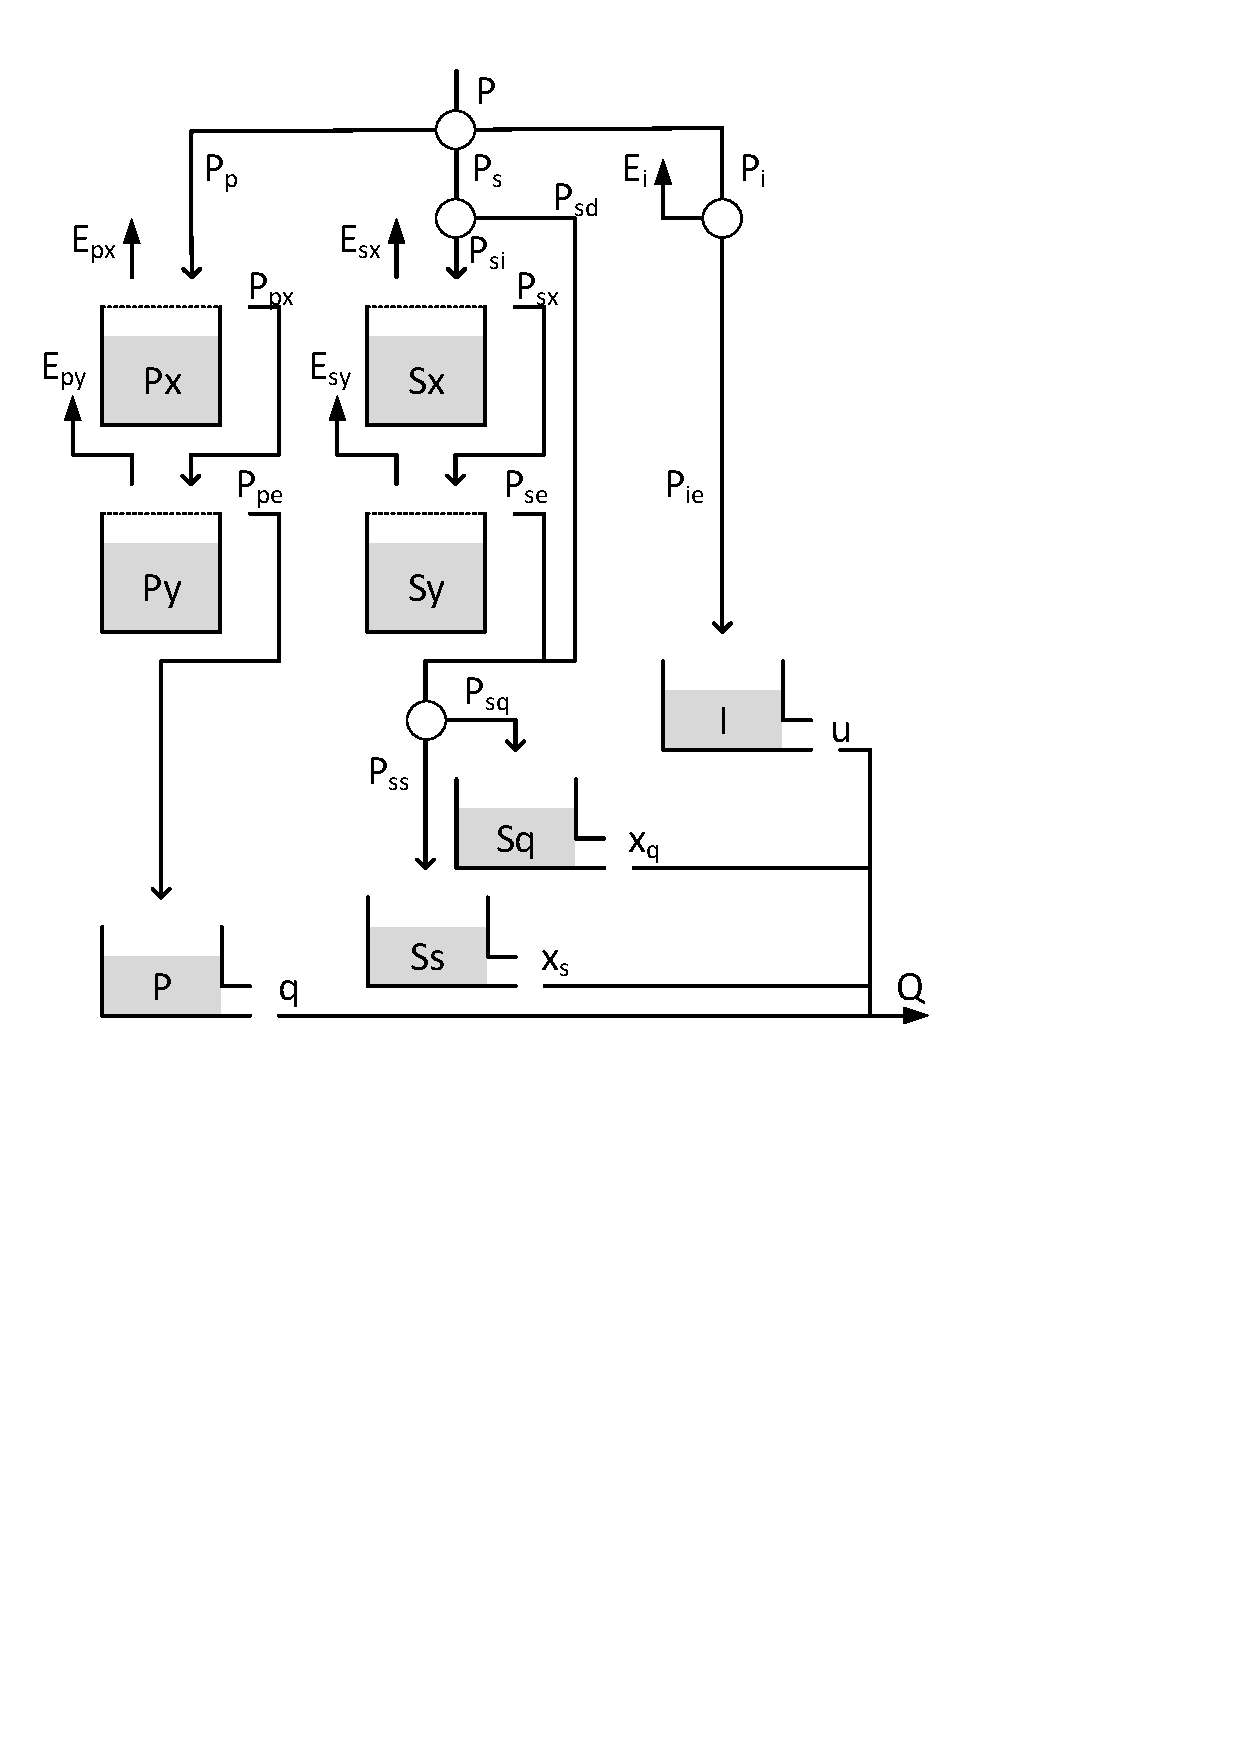
\includegraphics[trim=1cm 12cm 7cm 1cm,width=7cm,keepaspectratio]{./AppA_files/46_schematic.pdf}
\caption{Structure of the CLASSIC model} \label{fig:46_schematic}
\end{wrapfigure}

% permeable soils

\begin{align}
	\frac{dP_x}{dt} &= P_p-E_{px}-P_{px} \\
	P_p &= f_{ap} * P\\
	E_{px} &= 
	\begin{cases}
		f_{ap}*E_p, & \text{if } P_x > 0 \\
		0, & \text{otherwise}\\
	\end{cases}\\
	P_{px} &= 
	\begin{cases}
		P_p, & \text{if } P_x = f_{dp}*d_p \\
		0, & \text{otherwise}
	\end{cases}
\end{align}

Where $P_x$ [mm] is the current storage in the upper permeable layer, refilled by precipitation $P_p$ $[mm/d]$ and drained 

} % end of wrapfigure fix

\noindent 
$P_p$ is the fraction of precipitation $P$ $[mm/d]$ that falls on permeable area $f_{ap}$ [-].
$E_{px}$ occurs at the potential rate $E_p$ $[mm/d]$ whenever possible, adjusted for the fraction of area that is permeable soil.
$P_{px}$ only occurs when the store is at maximum capacity $f_{dp}*d_p$, where $d_p$ is the total soil depth (sum of depths X and Y) in the permeable area and $f_{dp}$ the fraction of this depth that is store X.

\begin{align}
	\frac{dP_y}{dt} &= -P_{px}+E_{py}+P_{pe} \\
	E_{py} &= 1.9*exp\left[{\frac{-0.6523*(P_y+f_{dp}*d_p)}{f_{dp}*d_p}}\right]*\left(f_{ap}*E_p - E_{px}\right)\\
	P_{pe} &= 
	\begin{cases}
		P_{px}, & \text{if } P_y = 0 \\
		0, & \text{otherwise}
	\end{cases}
\end{align}

Where $P_y$ [mm] is the current \emph{deficit}, which is increased by evaporation $E_{py}$ $[mm/d]$ and decreased by inflow $P_{px}$ $[mm/d]$.
Effective precipitation $P_{pe}$ $[mm/d]$ is only generated when the deficit is 0.
$E_{py}$ decreases exponentially with increasing deficit.

\begin{align}
	\frac{dP}{dt} &= P_{pe}-q \\
	q &= c_q*P
\end{align}

Where $P$ [mm] is the current storage in the permeable soil routing store, refilled by effective rainfall on permeable soil $P_{pe}$ $[mm/d]$ and drained by baseflow $q$ $[mm/d]$.
$q$ has a linear relation with storage through time scale parameter $c_p$ $[d^{-1}]$.

% semi-permeable soils
\begin{align}
	\frac{dS_x}{dt} &= P_{si}-E_{sx}-P_{sx} \\
	P_{si} &= d_1*P_s \\
	P_s &= f_{as}* P\\
	E_{sx} &= 
	\begin{cases}
		f_{as}*E_p, & \text{if } S_x > 0 \\
		0, & \text{otherwise}\\
	\end{cases}\\
	P_{sx} &= 
	\begin{cases}
		P_s, & \text{if } S_x = f_{ds}*d_s \\
		0, & \text{otherwise}
	\end{cases}
\end{align}

Where $S_x$ [mm] is the current storage in the upper semi-permeable layer, refilled by infiltration $P_{si}$ $[mm/d]$ and drained by evaporation $E_{sx}$ $[mm/d]$ and excess flow $P_{sx}$ $[mm/d]$.
$P_{si}$ is the fraction $d_1$ [-] of precipitation on semi-permeable area $P_s$ that infiltrates into the soil.
The complementary fraction $1-d_1$ of $P_s$ bypasses the soil and directly becomes effective rainfall as $P_{sd}$.
$P_s$ is the fraction of precipitation $P$ $[mm/d]$ that falls on semi-permeable area $f_{as}$ [-] .
$E_{sx}$ occurs at the potential rate $E_p$ $[mm/d]$ whenever possible, adjusted for the fraction of area that is semi-permeable soil.
$P_{sx}$ only occurs when the store is at maximum capacity $f_{ds}*d_s$, where $d_s$ is the total soil depth (sum of depths X and Y) in the semi-permeable area and $f_{ds}$ the fraction of this depth that is store X.

\begin{align}
	\frac{dS_y}{dt} &= -P_{sx}+E_{sy}+P_{se} \\
	E_{sy} &= 1.9*exp\left[{\frac{-0.6523*(S_y+f_{ds}*d_s)}{f_{ds}*d_s}}\right]*\left(f_{as}*E_p - E_{sx}\right)\\
	P_{pe} &= 
	\begin{cases}
		P_{sx}, & \text{if } S_y = 0 \\
		0, & \text{otherwise}
	\end{cases}
\end{align}

Where $S_y$ [mm] is the current \emph{deficit}, which is increased by evaporation $E_{sy}$ $[mm/d]$ and decreased by inflow $P_{sx}$ $[mm/d]$.
Effective precipitation $P_{se}$ $[mm/d]$ is only generated when the deficit is 0.
$E_{sy}$ decreases exponentially with increasing deficit.

\begin{align}
	\frac{dS_q}{dt} &= P_{sq}-x_q \\
	P_{sq} &= d_2*(P_{se}+P_{sd})\\	
	x_q &= c_{xq}*S_q
\end{align}

Where $S_q$ [mm] is the current storage in the semi-permeable quick soil routing store, refilled by a fraction of effective rainfall on semi-permeable soil $P_{sq}$ $[mm/d]$ and drained by quick flow $x_q$ $[mm/d]$.
$P_{sq}$ is the fraction $d_2$ [-] of $(P_{se}+P_{Sd})$ that is quick flow.
$x_q$ has a linear relation with storage through time scale parameter $c_{xq}$ $[d^{-1}]$.

\begin{align}
	\frac{dS_s}{dt} &= P_{ss}-x_s \\
	P_{ss} &= (1-d_2)*(P_{se}+P_{sd})\\	
	x_s &= c_{xs}*S_s
\end{align}

Where $S_s$ [mm] is the current storage in the semi-permeable quick soil routing store, refilled by a fraction of effective rainfall on semi-permeable soil $P_{ss}$ $[mm/d]$ and drained by slow flow $x_s$ $[mm/d]$.
$P_{ss}$ is the fraction $1-d_2$ [-] of $(P_{se}+P_{Sd})$ that is slow flow.
$x_s$ has a linear relation with storage through time scale parameter $c_{xs}$ $[d^{-1}]$.

%impermeable soils

\begin{align}
	\frac{dI}{dt} &= P_{ie}-u \\
	P_{ie} &= P_i-E_i\\
	P_i &= P-P_p-P_s\\
	u &= c_{u}*I
\end{align}

Where $I$ [mm] is the current storage in the impermeable soil routing store, refilled by effective rainfall on impermeable soil $P_{ie}$ $[mm/d]$ and drained by baseflow $u$ $[mm/d]$.
$P_{ie}$ is the remained of precipitation on impermeable soils $P_i$ $[mm/d]$, after a constant evaporation $E_i$ has been extracted.
$E_i$ is fixed at 0.5 $[mm/d]$.
$x_s$ has a linear relation with storage through time scale parameter $c_{xs}$ $[d^{-1}]$.
Total flow:

\begin{align}
	Q = q+x_s+x_q+u
\end{align}

\subsection{Parameter overview}
% Table generated by Excel2LaTeX from sheet 'Sheet1'
\begin{table}[htbp]
  \centering
    \begin{tabular}{lll}
    \toprule
    Parameter & Unit  & Description \\
    \midrule
    $f_{ap}$ & $-$   & Fraction permeable area \\
    $f_{dp}$ & $-$   & Store depth as fraction of $d_p$ \\
    $d_p$ & $mm$  & Total storage of Px and Py \\
    $c_q$ & $d^{-1}$ & Runoff coefficient \\
    $d_1$ & $-$   & Fraction of precipitation on semi-permeable area to Sx \\
    $f_{as}$ & $-$   & Fraction semi-permeable area \\
    $f_{ds}$ & $-$   & Store depth as fraction of $d_s$ \\
    $d_s$ & $mm$  & Total storage of Sx and Sy \\
    $d_2$ & $-$   & Fraction of semi-permeable area subsurface flow that is quick flow \\
    $c_{xq}$ & $d^{-1}$ & Runoff coefficient \\
    $c_{xs}$ & $d^{-1}$ & Runoff coefficient \\
    $c_{u}$ & $d^{-1}$ & Runoff coefficient \\
    \bottomrule
    \end{tabular}%
  \label{tab:addlabel}%
\end{table}%
